\section{RQ1: Predicting trip attraction with spatial features}
\subsubsection*{Prediction model evaluation and selection}

As previously explained, the choice of a suitable machine learning model is critical as Machine Learning explanation techniques such as SHAP would be less insightful if the predictions produced high inaccuracies. The evaluation results in Table \ref{tab:modeleval} show that the Gradient Boosting tree-based model (XGBoost) outperforms the other models in predicting the target variable Total arrivals (log), achieving an $R^2$ of 0.792, and outperforms itself when predicting the pre-transformed target variable Total arrivals with an $R^2$ of 0.633. Meanwhile, the simple Linear Regression model performs more poorly in comparison through underfitting (i.e., consistently low accuracy with training data folds), and the Multilayer Perceptron Artificial Neural Network model also performs poorly but due to overfitting (i.e., high accuracy achieved with training data folds but low accuracy with validation data folds). This shows that while XGBoost has long been popular thanks to its fast convergence and high validation accuracy, transforming the highly right-skewed target variable is another way to improve prediction performance. 

\begin{table}[ht]
    \centering
    \renewcommand{\arraystretch}{1.5}
    \begin{tabular}{|c|c|c|}
        \hline
        \rowcolor{lightgray}
        \textbf{Model} & \textbf{$R^2$ (raw)} & \textbf{$R^2$ (log)} \\
        \hline
        Linear Regression & 0.576 & 0.697 \\
        \rowcolor{pink}
        XGBoost & 0.633 & \textbf{0.792} \\
        ANN & 0.526 & 0.410\\
        \hline
    \end{tabular}
    \captionsetup{justification=centering}
    \caption{Comparing model $R^2$ results of 3 models predicting \\Total arrivals (raw) and Total arrivals (log) \\using spatial k-fold cross-validation}
    \label{tab:modeleval}
\end{table}

\begin{table}[hb]
    \centering
    \renewcommand{\arraystretch}{1.5}
    \begin{tabular}{|c|c|c|c|}
        \hline
        \rowcolor{lightgray}
        \textbf{Timeband} & \textbf{R$^2$} & \textbf{MSE} & \textbf{MAE} \\
        \hline
        Total   & \textbf{0.823} & 0.687 & 0.570 \\
        Morning & \textbf{0.809} & 0.614 & 0.571 \\
        Midday  & \textbf{0.828} & 0.629 & 0.549 \\
        Evening & \textbf{0.819} & 0.687 & 0.593 \\
        Late    & \textbf{0.824} & 0.635 & 0.601 \\
        \hline
    \end{tabular}
    \captionsetup{justification=centering}
    \caption{Finetuned XGBoost model evaluation results for \\All target variables (log) using nested spatial k-fold cross-validation}
    \label{tab:modelevaltimeband}
\end{table}

\begin{figure}[ht]
    \centering
    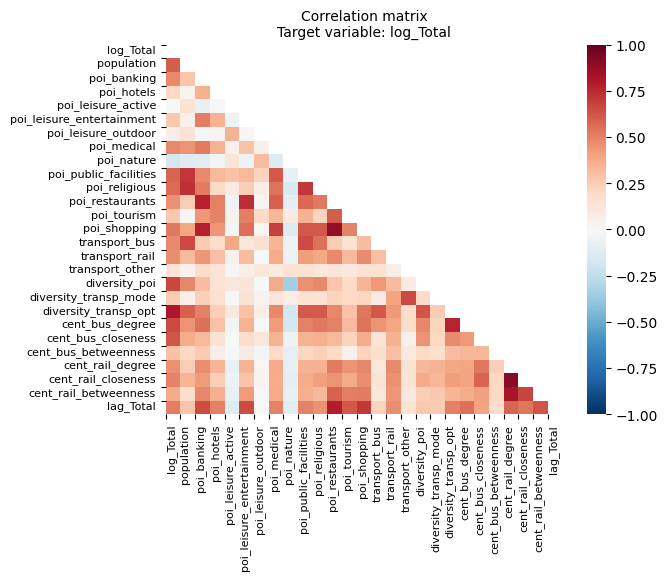
\includegraphics[width=0.8\textwidth]{correlation.png}
    \captionsetup{justification=centering}
    \caption{Correlation matrix of the input features and target variable Total arrivals (log)}
    \label{fig:corrmatt}
\end{figure}

On managing overfitting risks, XGBoost is a standout among other models also for its built-in L1 and L2 regularisation hyperparameters, which penalise the model for complexity and suppress highly correlated input features. This is particularly important when considering the complex patterns of correlations among our input features, as shown in Figure \ref{fig:corrmatt}. Here we observe a few cohorts of highly correlated features such as Population-Public Facilities-Religious POIs, Entertainment-Restautants-Shopping POIs, or among the different public transport centrality measures. Therefore, with XGBoost, we had the opportunity to further fine-tune two hyperparameters \textit{alpha} and \textit{lambda}---which represent L1 and L2 regularisation thresholds, respectively---to achieve even better results. Similar to previously, nested spatial k-fold cross-validation was used to fine-tune the model and validate the results. The fine-tuned XGBoost model improves $R^2$ up to \textbf{0.823} (an approx. 3pp increase) in predicting total arrivals from the pre-tuned model and performs consistently well in predicting arrivals by time band, as shown in Table \ref{tab:modelevaltimeband}. 

The results suggest that the fine-tuned XGBoost model is fit for purpose and enables us to address the first research question: ztextit{Built environment features are adequate predictors of public transport inflow demand in London to a high degree of accuracy}. This has implications for urban analytics literature and is important for urban planners and policymakers, as it provides a tool that can be used to predict public transport demand and plan for future infrastructure development that relies entirely on accessible data sources such as OpenStreetMap and the UK Census.

Before further analysis, it is important to recognise where the model falls short and what that may tell us about its potential lack of generalisability. Figure \ref{fig:outliers} shows the distribution of observations whose prediction residuals are 'outliers', i.e., the target variables are significantly overpredicted or underpredicted. These are mostly concentrated in Outer London where poor predictions go in both directions. While it is not easy to unravel, there are some possible root causes: 

\begin{itemize}
    \setlength\itemsep{0em}
    \item \textit{Low Spatial Autocorrelation:} There is some consistency between areas with low spatial autocorrelation of the target variable (see Figure \ref{fig:lisacluster}, grey regions), and where the model predicts more poorly. This may indicate incorporating spatial lag as a feature does improve the model's performance only where the spatial autocorrelation is present. In its absence, the model has a higher chance of poorer predictions based on other spatial features alone.
    \item \textit{Omitted features:} It is possible that adding variables such as car ownership and socioeconomic factors can help the model distinguish two hypothetical areas with the same built environment profiles but different public transport usage. This is especially true in Outer London, where car ownership is higher, and public transport services are less frequent.
    \item \textit{Incomplete target variable:} It is probable that a spatial unit with its built environment profile does have the predicted public transport trip attractiveness in reality. However, since only data from TfL-operated services are considered, omitting trip data from other operators more prevalent in Outer London and especially south of the Thames, it may show up as having an apparent overprediction. 
\end{itemize}

\begin{figure}[ht]
    \centering
    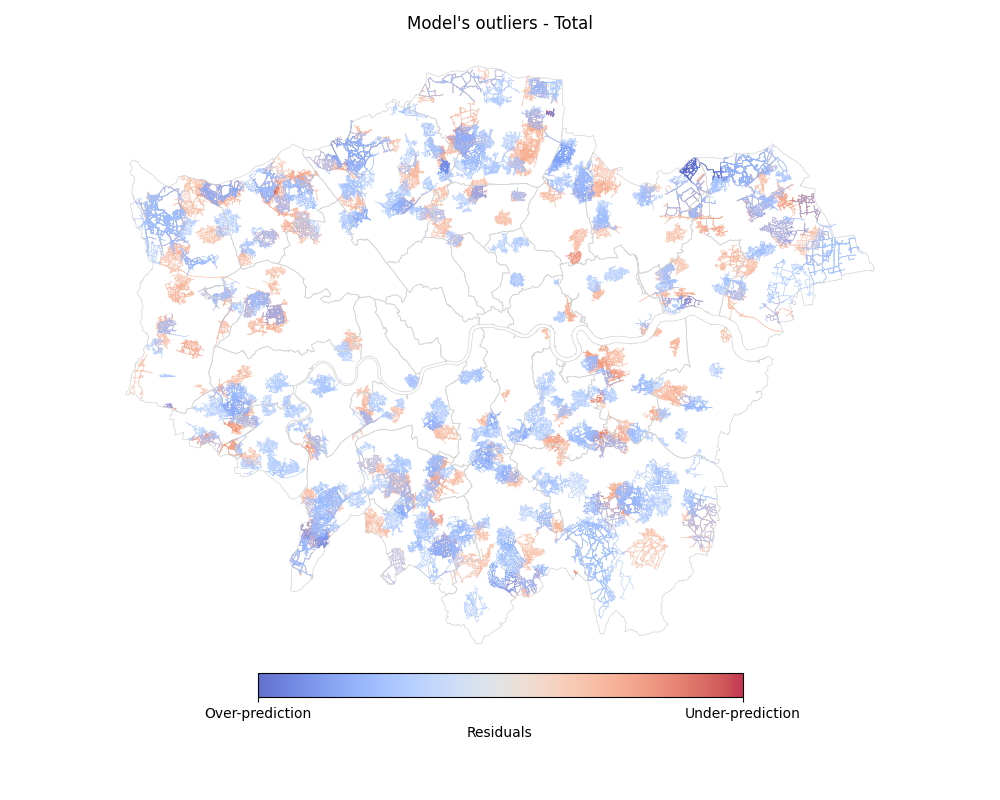
\includegraphics[width=0.8\textwidth]{outliers.png}
    \captionsetup{justification=centering}
    \caption{Observations with significant overprediction and underprediction (N=576 of 16,890)\\Fine-tuned XGBoost model, Total arrivals (log)}
    \label{fig:outliers}
\end{figure}

Nonetheless, these 'outliers' account for less than 3.5\% of the total observations, and the model's performance is still satisfactory in explaining the large majority of the spatial units in the Greater London area. Of course, due care is advised when applying the model directly to other localities, and further developments with more comprehensive datasets and additional features may be necessary.

\subsubsection*{Global feature importance}

After fitting the fine-tuned XGBoost model to the entire dataset, we applied interventional SHAP to obtain the SHAP values for each feature and observation. This allows us to evaluate the importance of each feature in predicting the target variable and understand the direction of the relationship between the feature and the target variable. 

Figure \ref{fig:beeswarmtotal} shows the summary of feature importance for the target variable Total arrivals (log) in order. First, it is evident that the connectivity profile features have outsized importance with the \textit{transport route option diversity index (diversity\_transp\_opt)} on top in predicting trip attractiveness. This is consistent with the reality that people tend to alight/exit at transport-rich areas where they have multiple bus routes or rail services for onward journeys, representing the interchange behaviour. The second most important feature is the spatial lag of the target variable (i.e., mean of target variables of neighbouring), which partially corroborates its influence to the model's performance hypothesised earlier when analysing. The most important amenity POI feature is \textit{shopping POIs}, which is also consistently important across all time bands (see Figure \ref{fig:beeswarmtimeband} in Appendix), followed by \textit{banking POIs}, \textit{active leisure POIs}, \textit{medical POIs}, and \textit{restaurant POIs}.

\begin{figure}[!ht]
    \centering
    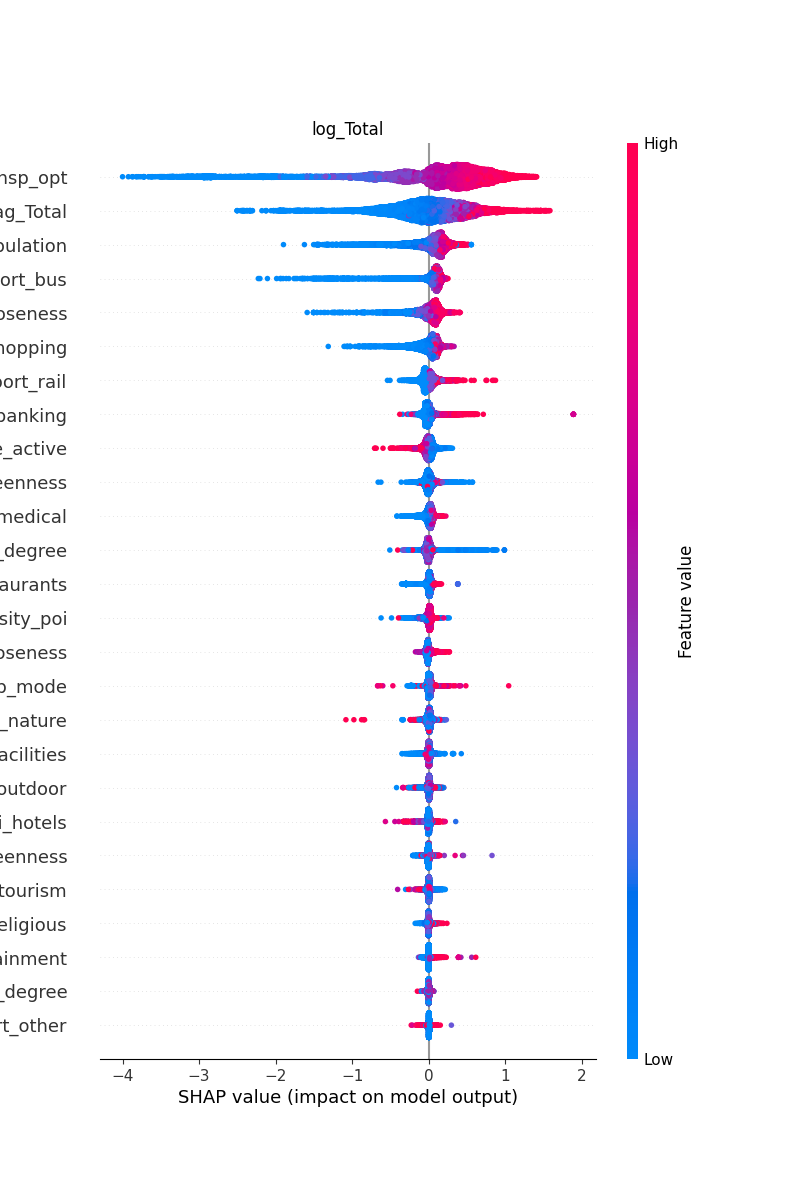
\includegraphics[width=0.8\textwidth]{beeswarm_log_Total.png}
    \captionsetup{justification=centering}
    \caption{Summary of feature importance based on SHAP values of a sample. Red-Blue scale represents the feature value, and the x-axis represents the SHAP value, i.e., impact on final model prediction of Total arrivals (log)}
    \label{fig:beeswarmtotal}
\end{figure}

This may seem counterintuitive at first that banking POIs are deemed more important in predicting trip attractiveness on a Saturday, but it is important to consider (1) the correlation between the input features as previously observed and (2) how the XGBoost model learns. Although regularisation is in place to suppress highly correlated features to cause overfitting, it does not drop them from the model. Consequently, when SHAP is applied for a retroactive explanation, highly correlated features will show comparable importance. In such cases, it is, therefore, more insightful to consider the SHAP values of the correlated features in clusters, as shown in Figure \ref{fig:barclustertotal}. We can see that there are differences from the previous graph that shows the order of importance of the features ( or feature clusters) in explaining trip attraction to an area as follows:

\begin{enumerate}
    \setlength\itemsep{0em}
    \item Transport route option diversity index
    \item Spatial Lag of Total arrivals (log)
    \item Population + Public Facilities
    \item Bus stop density + Bus stop closeness centrality (interchange hubs)
    \item Density of Shopping, Banking and Restaurants POIs
    \item Rail station and other transport node density
    \item Others
\end{enumerate}

\begin{figure}[!ht]
    \centering
    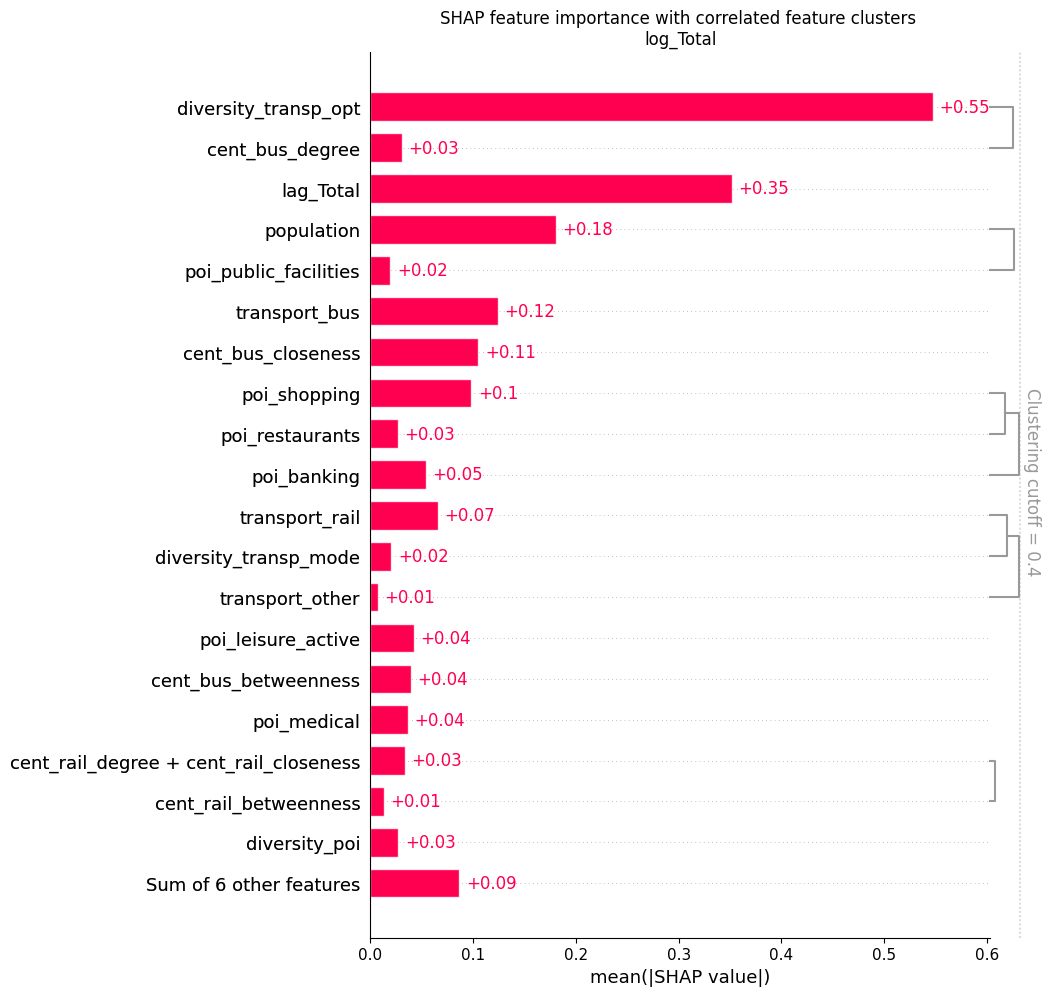
\includegraphics[width=0.8\textwidth]{new_barclus_log_Total.png}
    \captionsetup{justification=centering}
    \caption{Feature importance in predicting Total arrivals (log)\\ Features clustered by correlation and ordered by mean absolute SHAP values}
    \label{fig:barclustertotal}
\end{figure}

In summary, as it pertains to our first research question, the global feature importance analysis shows that built environment features are indeed important predictors of public transport inflow demand in London and that the XGBoost model is able to capture the complex relationships between these features and the target variable with high accuracy (>80\%). There are also opportunities to improve the prediction performance by addressing possibly omitted spatial and non-spatial features. The high importance of spatial lag feature is both an advantage and a shortcoming: While it drastically improves the model's performance overall, it penalises the model in areas where the spatial autocorrelation is low, reducing its generalisability to predicting the trip attractiveness of an area in isolation without considering its neighbours. Finally, highly correlated features should be considered in clusters when analysing importance to avoid interpreting undue importance to a single feature.

\section{RQ2: Local ML explanation for spatial analytics}

One of the highlights of SHAP is its ability to provide local explanations for individual predictions. In the case of a spatial system, these local explanations provide additional insights on spatial phenomena that are not well captured in a global feature importance analysis, namely spatial heterogeneity (i.e., varying impact of the target variable across different spatial units) and spatial non-stationarity (i.e., varying impact of an input feature on the target variable across different spatial units). SHAP's additive property allows us also to decompose the prediction of a spatial unit into the sum of the SHAP values of each feature and exact the contribution of each feature to the prediction.

Figure \ref{fig:localshap} shows the local SHAP values for two spatial units, Kew Gardens and Covent Garden, for a closer look. They represent two distinct localities with supposedly different amenity, transportation and trip attractiveness profiles. Kew Gardens is a relatively quiet but well-connected residential area in the public transport network, also known for its many renowned parks and gardens, while Covent Garden is a bustling commercial and entertainment district with high connectivity in the public transport network. The SHAP values for Kew Gardens show that the high importance of the spatial lag feature is due to the high number of public facilities and population in the area, which is consistent with the feature importance analysis. The SHAP values for Covent Garden show that the high importance of the shopping POIs feature is due to the high density of shopping amenities in the area, which is also consistent with the feature importance analysis.

\begin{figure}[!ht]
    \centering
    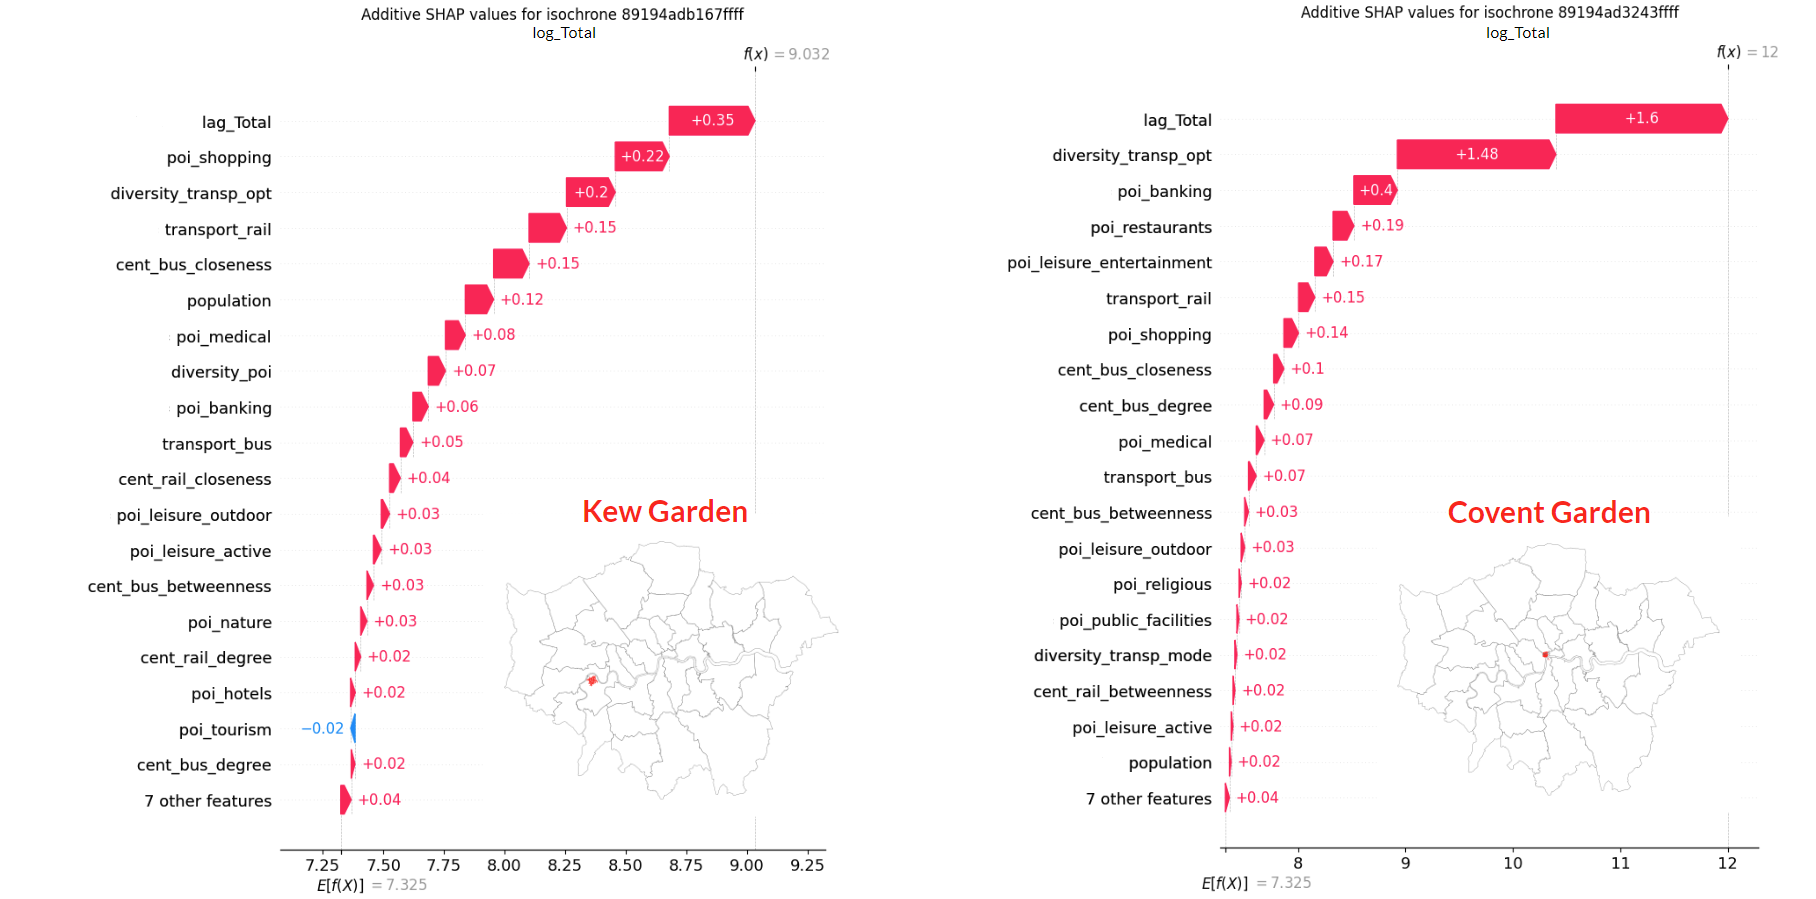
\includegraphics[width=\textwidth]{localshap.png}
    \captionsetup{justification=centering}
    \caption{Local SHAP values for 2 spatial units\\Kew Gardens and Covent Garden}
    \label{fig:localshap}
\end{figure}



\begin{figure}[!ht]
    \centering
    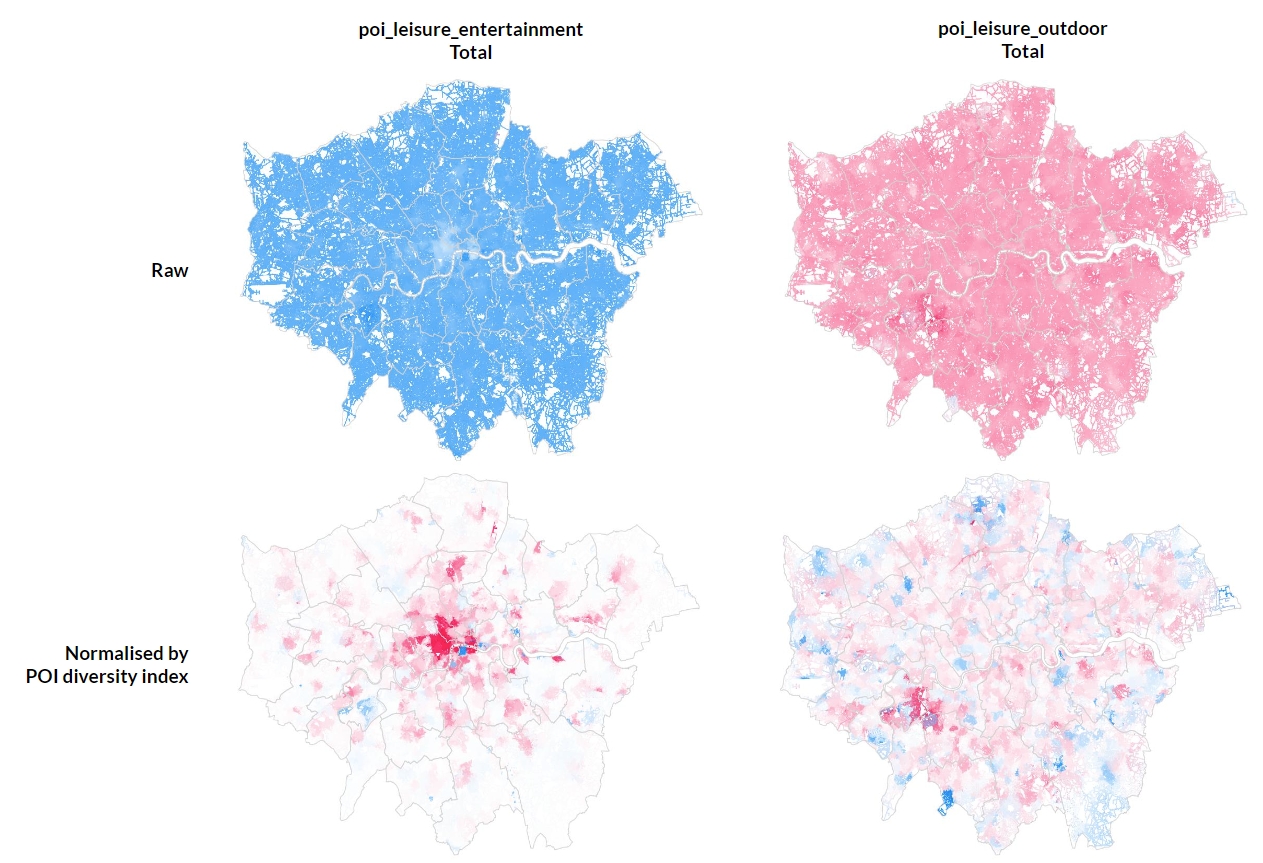
\includegraphics[width=\textwidth]{shaprawweighted.png}
    \captionsetup{justification=centering}
    \caption{Raw vs. weighted SHAP for 2 features\\Outdoor leisure POIs and Entertainment leisure POIs \\Total arrivals (log)}
    \label{fig:shaprawweighted}
\end{figure}

\begin{figure}[!ht]
    \centering
    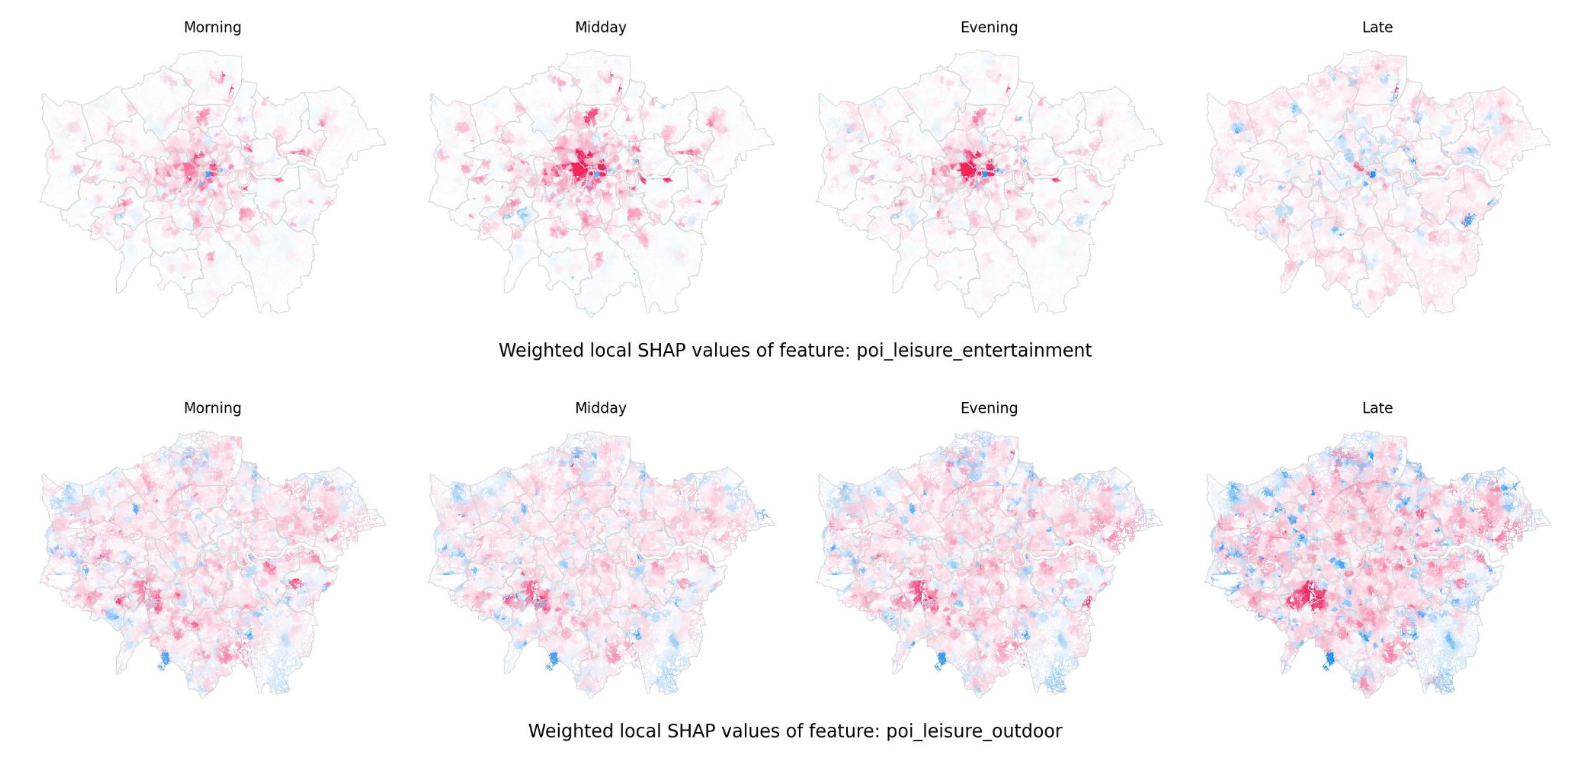
\includegraphics[width=\textwidth]{shaprawweightedtimeband.png}
    \captionsetup{justification=centering}
    \caption{Hot spots\\Arrivals by time band (log)}
    \label{fig:shaprawweightedtimeband}
\end{figure}